%==============================================================================
%== template for LATEX poster =================================================
%==============================================================================
%
%--A0 beamer slide-------------------------------------------------------------
\documentclass[final]{beamer}
\usepackage[orientation=portrait,size=a0,
            scale=1.25         % font scale factor
           ]{beamerposter}
           
\geometry{
  hmargin=2.5cm, % little modification of margins
}
\usepackage{booktabs}
\usepackage{makecell}
\usepackage{subcaption}
\usepackage[utf8]{inputenc}
\usepackage{csquotes}
\usepackage[english]{babel}
\usepackage[backend=biber,style=numeric-comp,sorting=none]{biblatex}
\AtBeginBibliography{\small}

\begin{filecontents*}{bib.bib}
@article{magani2021analysis,
    title = {Analysis of Multiplex Social Networks with {R}},
    author = {Matteo Magnani and Luca Rossi and Davide Vega},
    journal = {Journal of Statistical Software},
    year = {2021},
    volume = {98},
    number = {8},
    pages = {1--30},
  }
  @inproceedings{afsarmanesh2018partial,
  title={Partial and overlapping community detection in multiplex social networks},
  author={Afsarmanesh Tehrani, Nazanin and Magnani, Matteo},
  booktitle={{International Conference on Social Informatics}},
  pages={15--28},
  year={2018},
  organization={Springer}
}
@article{chesbrough2018value,
  title={Value creation and value capture in open innovation},
  author={Chesbrough, Henry and Lettl, Christopher and Ritter, Thomas},
  journal={Journal of Product Innovation Management},
  volume={35},
  number={6},
  pages={930--938},
  year={2018},
}
@article{mcevily2011measuring
,	author	= {McEvily, Bill and Tortoriello, Marco}
,	title	= {Measuring trust in organisational research: Review and recommendations}
,	journal	= {Journal of Trust Research}
,	year	= {2011}
,	volume	= {1}
,	number	= {1}
,	pages	= {23--63}
,	publisher	= {Taylor & Francis}
}
@article{levin2004strength
,	author	= {Levin, Daniel Z and Cross, Rob}
,	title	= {The strength of weak ties you can trust: The mediating role of trust in effective knowledge transfer}
,	journal	= {Management Science}
,	year	= {2004}
,	volume	= {50}
,	number	= {11}
,	pages	= {1477--1490}
,	publisher	= {Informs}
}
@article{van2017innovation,
  title={The innovation journey: you can't control it, but you can learn to maneuver it},
  author={Van de Ven, Andrew H},
  journal={Innovation},
  volume={19},
  number={1},
  pages={39--42},
  year={2017},
  publisher={Taylor \& Francis}
}
@book{van2008innovation
,	author	= {van de Ven, A and Polley, AH and DE, Garud, R and Venkataraman, S}
,	title	= {The Innovation Journey}
,	publisher	= {Oxford University Press}
,	year	= {2008}
}
\end{filecontents*}

\addbibresource{bib.bib}

\linespread{1.15}
%
%==The poster style============================================================
\usetheme{sharelatex}

%==Title, date and authors of the poster=======================================
\title
[Sunbelt 2022 Conference, Cairns, Australia] % Conference
{ % Poster title
Multilayer Network Perspective of Three Open Innovation Partnerships
}

\author{ % Authors
Ian Elsum\inst{1,3}, Andrew Terhorst\inst{2}
}
\institute
[Very Large University] % General University
{
\inst{1} Swinburne University of Technology, Melbourne, Australia\\[0.3ex]
\inst{2} Commonwealth Scientific and Industrial Research Organisation, Hobart, Australia\\[0.3ex]
\inst{3} Australian National University, Canberra, Australia
}
%\date{\today}

\begin{document}
\begin{frame}[t]
%==============================================================================
\begin{multicols}{3}
%==============================================================================
%==The poster content==========================================================
%==============================================================================

\section{Introduction}

Open innovation (OI) involves the exchange of existing, and creation of new, knowledge between business partners and use of this knowledge to achieve a specific innovation outcome within a market-relevant time frame \cite{chesbrough2018value}. An OI partnership is a type of temporary organisation: achieving a successful outcome depends on collective learning in the face of uncertainty and a range of social factors such as prior history of working together, individual personalities, and the balance of power and trust relations.\\~\

A multilayer network is a model used to represent multiple modes of interaction or relationships among entities of the same type. We used multilayer network analysis to investigate three OI partnerships to understand which relationships really count. Our analysis reveals that affect-based and cognition-based trust ties play a crucial role in OI. 

\section{Methods}

We investigated social interaction in three OI partnerships (Table \ref{tab:partnerships}). Participants from each partnership answered a set of name-generator and name-interpreter questions via an online survey. Their responses allowed us to construct eight directed network layers for each partnership: tacit and explicit knowledge provider, idea contributor, ideas realized with, affect-based and cognition-based trust, prior relationship with, and direct reports.

% \vskip1ex
% \begin{table}[]
% \centering
% \caption{Distinguishing features of each OI partnership.}
% \label{tab:partnerships}
% \resizebox{0.3\textwidth}{!}{%
% \begin{tabular}{@{}clccccc@{}}
% \toprule
% Partnership & Description & Archetype & Complexity & Stage & Partners & Participants \\ \midrule
% 1 & Improve cold-chain practices & Inbound & Low & Early & 7 & 18  \\
% 2 & Autonomous dairy farming & Coupled & High & Late & 8 & 25 \\
% 3 & Coordinated honeybee research & Outbound & Mod. & Early & 15 & 40 \\ \bottomrule
% \end{tabular}%
% }
% \end{table}
% \vskip2ex

\vskip1ex
\begin{table}[]
\centering
\caption{Distinguishing features of each OI partnership.}
\label{tab:partnerships}
\resizebox{0.29\textwidth}{!}{%
\begin{tabular}{@{}cllc@{}}
\toprule
Partnership & Novelty & Level of Uncertainty & Stage \\ \midrule
1 & \makecell[tl]{Incremental changes \\to existing practices.} & \makecell[tl]{Low, few unknown \\unknowns.} & Forming \\
2 & \makecell[tl]{Radical changes to \\existing practices.} & \makecell[tl]{Transitioning from \\extremely high to low \\as ideas are \\implemented.} & Finishing  \\
3 & \makecell[tl]{New ways of doing, \\so high.} & \makecell[tl]{High, many unknown \\unknowns.} & Initiation \\ \bottomrule
\end{tabular}%
}
\end{table}
\vskip2ex

The multilayer network analysis was carried out using the \texttt{multinet} package in \texttt{R} \cite{magani2021analysis}. We are interested in what binds small communities of practice in OI partnerships. Our analysis focused on community structures spanning multiple network layers. We used the clique percolation algorithm to detect communities. This algorithm assumes communities consist of small groups of tightly connected actors (cliques) adjacent to each other. With multilayer networks, we are interested in cliques that share multiple edge types \cite{afsarmanesh2018partial}. In our analysis, we identified communities with adjacent cliques of three or more actors sharing edges across four network layers.

\section{Results}

% Table \ref{tab:sum_stats} presents summary statistics for each multilayer network.

% \vskip1ex
% \begin{table}[h]
% \tiny
% \begin{subtable}[h]{0.25\textwidth}
% \centering
% \begin{tabular}{lrrrrrrrrr}
% \toprule
% Network & n & m & dir & nc & slc & dens & cc & apl & dia \\ 
% \midrule
% Tacit knowledge provider &  15 &  26 &   1 &   1 &  15 & 0.12 & 0.40 & 1.72 &   3 \\ 
% Explicit knowledge provider &  18 &  61 &   1 &   1 &  18 & 0.20 & 0.47 & 2.05 &   4 \\
% Idea contributor &  17 &  53 &   1 &   1 &  17 & 0.19 & 0.48 & 2.73 &   7 \\ 
% Ideas realized with &  18 &  49 &   1 &   1 &  18 & 0.16 & 0.38 & 2.15 &   5 \\ 
% Affect-based trust &  18 &  46 &   1 &   1 &  18 & 0.15 & 0.35 & 1.97 &   4 \\ 
% Cognition-based trust &  18 &  79 &   1 &   1 &  18 & 0.26 & 0.49 & 1.79 &   3 \\ 
% Worked previously with &  17 &  55 &   1 &   2 &  13 & 0.20 & 0.58 & 1.83 &   4 \\ 
% Report to &  16 &  32 &   1 &   1 &  16 & 0.13 & 0.30 & 1.79 &   3 \\ 
% \_flat\_ &  18 & 401 &   1 &   1 &  18 & 1.31 & 0.57 & 1.65 &   2 \\ 
% \bottomrule
% \end{tabular}
% \caption{Partnership 1}
% \label{tab:p1}
% \end{subtable}
% \vfill
% \begin{subtable}[h]{0.25\textwidth}
% \centering
% \begin{tabular}{lrrrrrrrrr}
% \toprule
% Layer & n & m & dir & nc & slc & dens & cc & apl & dia \\ 
% \midrule
% Tacit knowledge provider &  24 & 136 &   1 &   1 &  24 & 0.25 & 0.60 & 1.96 &   5 \\ 
% Explicit knowledge provider &  25 & 105 &   1 &   1 &  25 & 0.18 & 0.40 & 2.23 &   5 \\
% Idea contributor &  25 & 141 &   1 &   1 &  25 & 0.23 & 0.53 & 1.84 &   3 \\ 
% Ideas realized with &  22 & 111 &   1 &   1 &  22 & 0.24 & 0.54 & 1.94 &   4 \\ 
% Affect-based trust &  25 & 143 &   1 &   1 &  25 & 0.24 & 0.60 & 1.99 &   4 \\ 
% Cognition-based trust &  25 & 206 &   1 &   1 &  25 & 0.34 & 0.64 & 1.76 &   4 \\ 
% Worked previously with &  25 & 151 &   1 &   1 &  25 & 0.25 & 0.53 & 2.05 &   4 \\ 
% Report to &  20 &  41 &   1 &   1 &  20 & 0.11 & 0.44 & 1.56 &   3 \\ 
% \_flat\_ &  25 & 1034 &   1 &   1 &  25 & 1.72 & 0.78 & 1.44 &   3 \\ 
% \bottomrule
% \end{tabular}
% \caption{Partnership 2}
% \label{tab:p2}
% \end{subtable}
% \vfill
% \begin{subtable}[h]{0.25\textwidth}
% \centering
% \begin{tabular}{lrrrrrrrrr}
% \toprule
% row & n & m & dir & nc & slc & dens & cc & apl & dia \\ 
% \midrule
% Tacit knowledge provider &  38 & 101 &   1 &   2 &  36 & 0.07 & 0.28 & 2.11 &   5 \\ 
% Explicit knowledge provider &  37 & 121 &   1 &   1 &  37 & 0.09 & 0.39 & 2.49 &   5 \\
% Idea contributor &  40 & 132 &   1 &   1 &  40 & 0.08 & 0.35 & 2.25 &   6 \\ 
% Ideas realized with &  33 &  76 &   1 &   3 &  26 & 0.07 & 0.24 & 1.89 &   3 \\ 
% Affect-based trust &  40 & 145 &   1 &   2 &  36 & 0.09 & 0.42 & 1.81 &   3 \\ 
% Cognition-based trust &  40 & 211 &   1 &   1 &  40 & 0.14 & 0.57 & 2.49 &   7 \\ 
% Worked previously with &  35 &  92 &   1 &   4 &  27 & 0.08 & 0.36 & 2.81 &   7 \\ 
% Report to &  33 &  47 &   1 &   2 &  31 & 0.04 & 0.15 & 1.52 &   4 \\ 
% \_flat\_ &  40 & 925 &   1 &   1 &  40 & 0.59 & 0.54 & 2.07 &   5 \\ 
% \bottomrule
% \end{tabular}
% \caption{Partnership 3}
% \label{tab:p2}
% \end{subtable}
% \caption{Descriptive statistics for each partnership.}
% \label{tab:sum_stats}
% \end{table}
% \vskip2ex
Figure \ref{fig:network} depicts multilayer communities overlaid onto the different network layers. Partners are distinguished by node color. Partnership 1 has only five distinct communities. Partnership 2, in contrast, has 19 distinct communities, many of which overlap, suggesting these communities have a common basis. Partnership 2 is also quite mature, which may explain the relative abundance of communities. Like Partnership 1, no community is associated with the explicit knowledge provider network. Partnership 3 has nine distinct communities, only some of which overlap.\\~\ 

Table \ref{tab:norm} shows which network layers feature prominently in each partnership's communities. Affect- and cognition-based trust feature strongly in all three partnerships. These two layers also tend to be closely associated with ideation and idea realization.
% add network diagrams here
\vskip1ex
\begin{figure}
\centering
\begin{subfigure}[b]{0.29\textwidth}
\centering
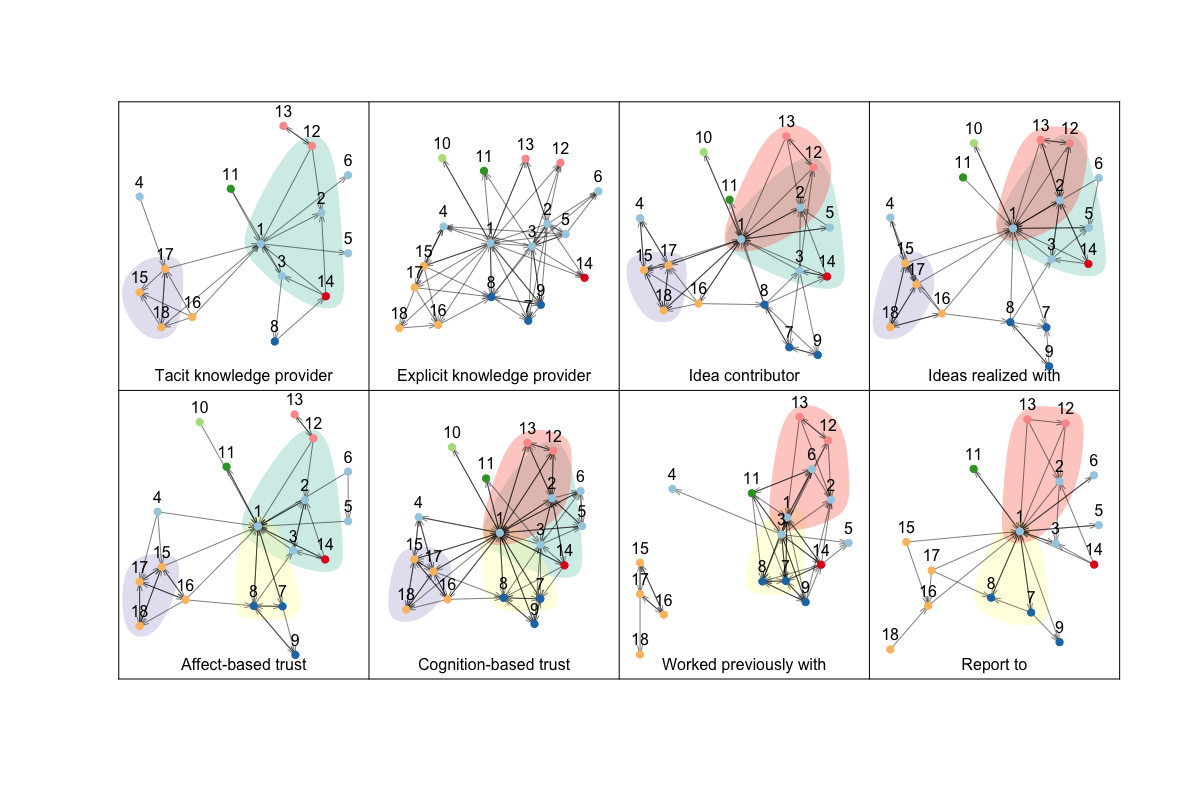
\includegraphics[width=\textwidth,trim={3cm 2.5cm 2.5cm 3cm},clip]{case_1.png}
\caption{Partnership 1}
\label{fig:p1}
\end{subfigure}
\hfill
\begin{subfigure}[b]{0.3\textwidth}
\centering
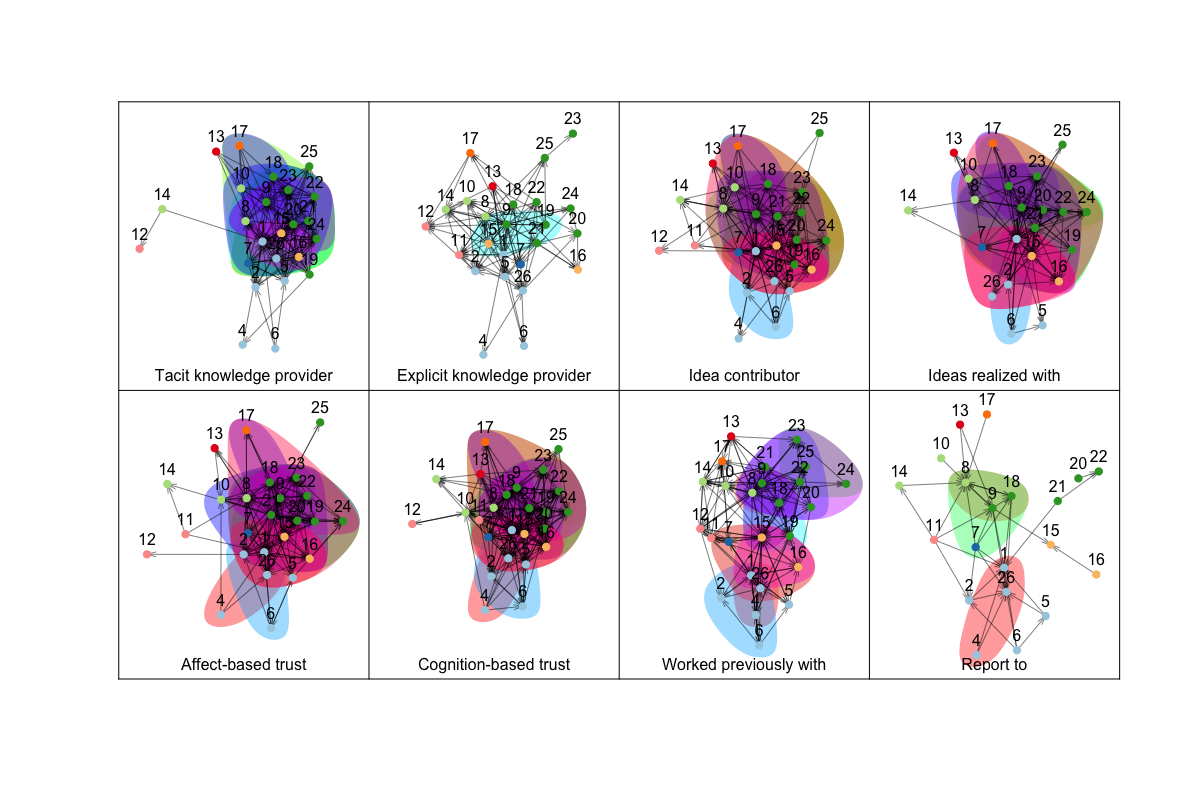
\includegraphics[width=\textwidth,trim={3cm 2.5cm 2.5cm 3cm},clip]{case_2.png}
\caption{Partnership 2}
\label{fig:p2}
\end{subfigure}
\hfill
\begin{subfigure}[b]{0.3\textwidth}
\centering
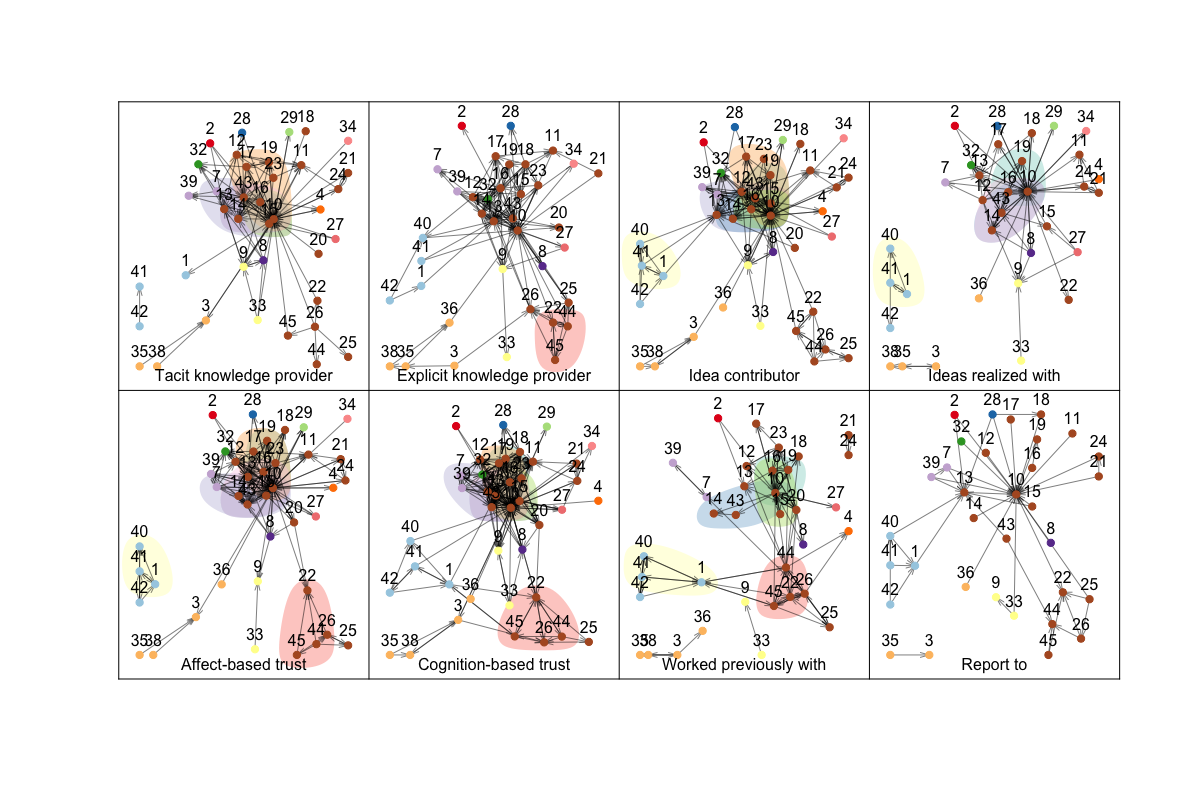
\includegraphics[width=\textwidth,trim={3cm 2.5cm 2.5cm 3cm},clip]{case_3}
\caption{Partnership 3}
\label{fig:p3}
\end{subfigure}
\caption{Multilayer communities in each partnership.}
\label{fig:network}
\end{figure}
\vskip2ex

\vskip1ex
\begin{table}[]
\centering
\caption{Relative dominance of network layers in each partnership (CID = number of detected communities).}
\label{tab:norm}
\resizebox{0.3\textwidth}{!}{%
\begin{tabular}{@{}lccc@{}}
\toprule
 & Partnership 1 & Partnership 2 & Partnership 3 \\
 & CID = 5 & CID = 19 & CID = 9 \\ \midrule
Tacit knowledge provider & 0.40 & 0.68 & 0.33 \\
Explicit knowledge provider & 0.00 & 0.00 & 0.44 \\
Idea contributor & 0.80 & 0.84 & 0.89 \\
Ideas realized with & 0.80 & 0.79 & 0.44 \\
Affect-based trust & 0.60 & 0.84 & 0.89 \\
Cognition-based trust & 1.00 & 1.00 & 0.89 \\
Worked previously with & 0.40 & 0.42 & 0.33 \\
Report to & 0.20 & 0.05 & 0.33 \\ \bottomrule
\end{tabular}
}
\end{table}
\vskip2ex

\section{Discussion}

\subsection{Role of affect- and cognition-based trust} 

Affect- and cognition-based trust play a critical role in almost all communities across the three partnerships (Table \ref{tab:norm}). We believe this is because trust is a pre-requisite for collective learning in a context of uncertainty. \\~\

Affect- and cognition-based trust are key factors influencing one crucial component of collective learning: willingness to provide and receive both explicit and tacit knowledge \cite{levin2004strength}. Another key component is how this knowledge is applied -- action is necessary for learning in a context of uncertainty \cite{van2008innovation}. However, uncertainty results in (a) people acting without the ability to predict the outcome of their action, and (b) \enquote{noisy} learning where people have to contend with ambiguous outcomes of action. In this context, trust is essential for willingness to act, with cognition-based trust playing a key role in deciding whether to act or not \cite{mcevily2011measuring}.  

\subsection{Novelty and stage of the innovation}

The higher the novelty of innovation, the greater the level of uncertainty. Tacit knowledge is more important for innovating in a context of high uncertainty \cite{van2008innovation}. A combination of high uncertainty and the late stage of the partnership may explain the prominence of the tacit knowledge provider network layer in Partnership 2. \\~\

The relative lack of importance of the \enquote{ideas realized with} network layer in Partnership 3 is likely a consequence of the early stage of this partnership, where the emphasis is on the formulation of ideas about what might be done rather than implementing them.

\section{Conclusion}

Our multilayer network analysis of different OI partnerships allowed us to see which layers count in OI. Affect- and cognition-based trust underpins knowledge sharing, ideation and idea realization in a context of the uncertainty inherent in innovation. Consequently, actions to build trust need to be incorporated into planning for and implementing OI partnerships and the development of trust-based communities of practice monitored as an indicator of the \enquote{health} of a partnership. 

%==============================================================================
%==End of content==============================================================
%==============================================================================

%--References------------------------------------------------------------------

\section{References}

\printbibliography[heading=none]

%--End of references-----------------------------------------------------------

\end{multicols}

%==============================================================================
\end{frame}
\end{document}
